\PassOptionsToPackage{table}{xcolor}
\documentclass[nobib,nofonts]{tufte-handout}

%\geometry{showframe} % display margins for debugging page layout

%%% MF additions
% \usepackage[table]{xcolor}
\usepackage[nographicx, nohyperref, nosubcaption, nogb4e, nobiblatex]{../99-auxiliary-files/00-mypackages}
\usepackage{../99-auxiliary-files/00-mycommands}
\usepackage{../99-auxiliary-files/00-myenvironments}

\usepackage{titlesec}
\usepackage{etoolbox}
\usepackage{tikz-qtree}
\usepackage{subcaption}

\usepackage{pgfplots}
% externalize PGF plots
% \usepgfplotslibrary{external}
% \tikzexternalize

% \titleformat{\section}
% {\large\bfshape}{\thesection}{1em}{}

\setcounter{secnumdepth}{5}
\renewcommand\thesection{\arabic{section}}

% this length controls tha hanging indent for titles
% change the value according to your needs
\newlength\titleindent
\setlength\titleindent{0.7cm}

\pretocmd{\paragraph}{\stepcounter{subsection}}{}{}
\pretocmd{\subparagraph}{\stepcounter{subsubsection}}{}{}

\titleformat{\chapter}[block]
  {\normalfont\huge\bfseries}{}{0pt}{\hspace*{-\titleindent}}

\titleformat{\section}
  {\normalfont\Large\itshape}{\llap{\parbox{\titleindent}{\thesection\hfill}}}{0em}{}

\titleformat{\subsection}
  {\normalfont\itshape}{\llap{\parbox{\titleindent}{\thesubsection\hfill}}}{0em}{}

\titleformat{\subsubsection}
  {\normalfont\normalsize\itshape}{\llap{\parbox{\titleindent}{\thesubsubsection}}}{0em}{}

\titleformat{\paragraph}[runin]
  {\normalfont\normalsize\itshape}{}{-0.7cm}{}[\xspace \ \ \ \ ]

\titleformat{\subparagraph}[runin]
  {\normalfont\normalsize}{\llap{\parbox{\titleindent}{\thesubsubsection\hfill}}}{0em}{}

\titlespacing*{\chapter}{0pt}{0pt}{20pt}
\titlespacing*{\subsubsection}{0pt}{3.25ex plus 1ex minus .2ex}{1.5ex plus .2ex}
\titlespacing*{\paragraph}{0pt}{3.25ex plus 1ex minus .2ex}{0em}
\titlespacing*{\subparagraph}{0pt}{3.25ex plus 1ex minus .2ex}{0em}

\DefineNamedColor{named}{mygray2}{cmyk}{0.55,0.25,0.25,0.25}
\newcommand{\mygray}[1]{\textcolor{mygray2}{#1}}

%%% Tufte style
\usepackage{graphicx} % allow embedded images
  \setkeys{Gin}{width=\linewidth,totalheight=\textheight,keepaspectratio}
  \graphicspath{{graphics/}} % set of paths to search for images

\usepackage{fancyvrb} % extended verbatim environments
  \fvset{fontsize=\normalsize}% default font size for fancy-verbatim environments

% Standardize command font styles and environments
\newcommand{\doccmd}[1]{\texttt{\textbackslash#1}}% command name -- adds backslash automatically
\newcommand{\docopt}[1]{\ensuremath{\langle}\textrm{\textit{#1}}\ensuremath{\rangle}}% optional command argument
\newcommand{\docarg}[1]{\textrm{\textit{#1}}}% (required) command argument
\newcommand{\docenv}[1]{\textsf{#1}}% environment name
\newcommand{\docpkg}[1]{\texttt{#1}}% package name
\newcommand{\doccls}[1]{\texttt{#1}}% document class name
\newcommand{\docclsopt}[1]{\texttt{#1}}% document class option name
\newenvironment{docspec}{\begin{quote}\noindent}{\end{quote}}% command specification environment

\newcommand{\proplog}{\acro{PropLog}}
\newcommand{\EFSQ}{\ensuremath{\mathit{EFSQ}}\xspace}

\renewcommand{\markdef}[1]{\emph{#1}}

%%%%%%%%%%%%%%%%%%%%%%%%%%%%%%%%%%%%%%%%%%%%%%%%%%

% \usepackage[sc,osf]{mathpazo}
% \linespread{1.05}


\title{Probability theory}

\author[M.~Franke]{Michael Franke}

\date{} % without \date command, current date is supplied

\usepackage{epsdice} % for dice

\newcommand{\mult}{\ensuremath{\cdot}}

\begin{document}

\maketitle

\begin{abstract}
\noindent
Basics of probability theory:
axiomatic definition,
interpretation,
joint distributions,
marginalization,
conditional probability,
Bayes rule,
stochastic independence.
Random variables \& expected values.
\end{abstract}


\noindent Classical logic explores which conclusions follow from a set of premises.
The conclusion must follow necessarily from the premises, based on the logical structure of the premises and the conclusions, not based on additional knowledge about the actual world, not on things that could (logically) have been different.

In contrast, much of human knowledge and reasoning revolves around \emph{statistical knowledge}: since most birds can fly, if I learn that Tweety is a bird, it is reasonable to conclude that Tweety is \emph{likely} to fly (unless I have more information about Tweety that might provide evidence against this uncertain inference).
Probability theory is a formal framework to capture such \emph{reasoning under uncertainty}.

Just like there are several logics, there are also several formalizations for reasoning with uncertainty, some of which are simpler and some of which are way more complex than standard probability theory.
Some alternative systems are argued to be more empirically adequate for capturing human reasoning than probability theory.
However, what singles out probability theory is that it strikes a good balance between simplicity, adequacy and applicability.
As such, it lies at the heart of much of modern statistics and machine learning, with a plethora of mathematical results and algorithms supporting its wide-spread applications in all areas of science.
% add some historical notes maybe in the margin?

\section{Probability}

The most central concept of probability theory is that of a probability distribution.
A probability distribution captures a state of uncertainty regarding which of a number of relevant events might hold or will occur.
It assigns a number to each relevant event.
This number indicates how likely the event is supposed to be (relative to others).

\subsection{Outcomes, events, observations}

We are interested in the space $\Omega$ of all \markdef{elementary outcomes} $\omega_1,
\omega_2, \dots$ of a process or event whose execution is (partially) random or
unknown. Elementary outcomes are mutually exclusive. The set $\Omega$ exhausts all
possibilities.\sidenote{For simplicity of exposure, we gloss over subtleties arising when
  dealing with infinite sets $\Omega$.}

\begin{example}
  The set of elementary outcomes of a single coin flip is $\Omega_{\text{coin flip}} =
  \set{\text{heads}, \text{tails}}$. The elementary outcomes of tossing a six-sided die is
  $\Omega_{\text{standard die}} = \set{\epsdice{1}, \epsdice{2}, \epsdice{3}, \epsdice{4},
    \epsdice{5}, \epsdice{6}}$.\sidenote{
    Think of $\Omega$ as a partition of the space of all possible worlds, i.e., ways in which the world could be, where we lump together into one partition cell all ways in which the world could be that are equivalent regarding those aspects of reality that we are interested in.
    We do not care whether the coin lands in the mud or in the sand.
    It only matters whether it came up heads or tails.
    Each elementary event can be realized in myriad ways.
    $\Omega$ is our, the modellers', first crude simplification of nature, abstracting away aspects we
    currently do not care about.
  }
\end{example}

An \markdef{event} $A$ is a subset of $\Omega$. Think of an event as a (possibly partial)
observation. We might observe, for instance, not the full outcome of tossing a die, but only
that there is a dot in the middle. This would correspond to the event
$A = \set{\epsdice{1}, \epsdice{3}, \epsdice{5}} \subseteq \Omega_{\text{standard die}}$,
i.e., observing an odd numbered outcome. The trivial observation $A = \Omega$ and the
impossible observation $A = \emptyset$ are counted as events, too. The latter is included for
technical reasons.


For any two events $A, B \subseteq \Omega$, standard set operations correspond to logical
connections in the usual way. For example, the conjunction $A \cap B$ is the observation of
both $A$ and $B$; the disjunction $A \cup B$ is the observation that it is either $A$ or $B$;
the negation of $A$, $\overline{A} = \set{\omega \in \Omega \mid \omega \not \in A}$, is the
observation that it is not $A$.

\subsection{Probability distributions}

A \markdef{probability distribution} $P$ over $\Omega$ is a function
$P \mycolon \pow{\Omega} \rightarrow \mathds{R}$ that assigns to all events
$A \subseteq \Omega$ a real number (from the unit interval, see A1), such that the following
(so-called Kolmogorov axioms) are satisfied:
\begin{enumerate}[{A}1.]
\item $0 \le P(A) \le 1$
\item $P(\Omega) = 1$
\item $P(A_1 \cup A_2 \cup A_3 \cup \dots) = P(A_1) + P(A_2) + P(A_3) + \dots $ \\
  whenever $A_1, A_2, A_3, \dots$ are mutually exclusive\sidenote{
  A3 is the axiom of \emph{countable additivity}.
  Finite additivity may be enough for finite or countable sets $\Omega$, but infinite additivity is necessary for full generality in the uncountable case.
  }
\end{enumerate}
Occasionally we encounter notation $P \in \Delta(\Omega)$ to express that $P$ is a probability
distribution over $\Omega$.\sidenote{E.g., in physics, theoretical economics or game
  theory. Less so in psychology or statistics.} If $\omega \in \Omega$ is an elementary event,
we often write $P(\omega)$ as a shorthand for $P(\set{\omega})$. In fact, if $\Omega$ is
finite, it suffices to assign probabilities to elementary outcomes.

It is possible for a probability distribution $P \in \Delta(\Omega)$ to assign probability zero $P(\omega) = 0$ for some $\omega \in \Omega$.
The set of elementary outcomes to which $P$ assigns positive probability is called the \emph{support} of $P$.

\subsection{Implications of the axiomatic definition}

A number of useful rules follows immediately from of this definition.
Here we prove one (see exercises for more).

\begin{claim}
  \label{theorem:sum-of-elementary-outcomes}
  If $\Omega = \set{\omega_{1}, \dots, \omega_{n}}$ is a finite set of elementary outcomes and $P \in \Delta(\Omega)$ a probability distribution over $\Omega$, then the sum of the probabilities of all elementary outcomes is equal to 1:
  \begin{align*}
    \sum_{i = 1}^{n} P(\omega_{i}) = 1
  \end{align*}
\end{claim}
\begin{proof}
  From A3 we know that:
  \begin{align*}
  \sum_{i = 1}^{n} P(\omega_{i}) = P(\set{w_{1}} \cup \dots \cup \set{w_{n}})
  \end{align*}
  Since $\Omega = \set{w_{1}} \cup \dots \cup \set{w_{n}}$, it follows from A2 that $\sum_{i = 1}^{n} P(\omega_{i}) = 1$.
\end{proof}

It follows from Claim~\ref{theorem:sum-of-elementary-outcomes} that, in order to fully determine a probability distribution $P \in \Delta(\Omega)$ over a finite $\Omega$ with $n$ elements, we only need to specify $n-1$ probabilities, since the $n$th probability can be retrieved as ``one minus the sum of all others.''

\subsection{Interpretations of probability}

It is reasonably safe, at least preliminarily, to think of probability, as defined above, as a
handy mathematical primitive which is useful for certain applications. There are at least three
ways of thinking about where this primitive probability might come from, roughly paraphrasable
like so:
\begin{enumerate}[1.]
\item \markdef{Frequentist:} Probabilities are generalizations of intuitions/facts about frequencies of events in
  repeated executions of a random event.
\item \markdef{Subjectivist:} Probabilities are subjective beliefs by an agent who is
  uncertain about the outcome of a random event.
\item \markdef{Realist:} Probabilities are a property of an intrinsically random world.
\end{enumerate}

While trying to stay away from philosophical quibbles, we will adopt a subjectivist interpretation of probabilities, since this interpretation is most encompassing and ---arguably--- intuitive.
But note that frequentist considerations should affect what a rational agent should believe (see the urns scenario in Section~\ref{sec:urns-frequencies}).

\begin{example}[Subjective beliefs about the weather]
  Consider the set of elementary outcomes $\Omega_{\text{weather}} = \set{\text{sunny}, \text{misty}, \text{rainy}}$ of potential weather condition for tomorrow at noon.\sidenote{
    We assume that these states are independent and that these are all the states the weather might be in (for simplicity of an example).
  }
Jones, the optimist, does not know what the weather will bring, but believes that it is most likely to be sunny.
In fact, Jones believes ---for whatever reason--- that it is three times as likely to be sunny than that it is going to be misty.
Jones also believes that being misty and being rainy is equallly likely.
This information about Jones' \emph{relative degrees of credence} alone, is enough to know that, according to Jones, the probability of the three weather conditions are given in the first line of Table~\ref{tab:beliefs-weather}.

Smith is more pessimistic.
Smith's believes that ``misty'' is twice as likely as ``sunny'' and that ``rainy'' is seven times more likely than ``sunny.''
This information about relative probabilities is enough to know that Smith's beliefs are those represented in the second line of Table~\ref{tab:beliefs-weather}.

Notice that, in the case of beliefs about the weather, it is fairly unproblematic to imagine that two agents, even rational ones, might have quite different (subjective) beliefs about the same set of elementary outcomes.
This is not always the case (see Section~\ref{sec:urns-frequencies}).

\begin{table}
  \centering
  \begin{tabular}{lccc}
    & sunny & cloudy & rainy \\ \midrule
    Jones' beliefs  & 0.6   & 0.2    & 0.2   \\
    Smith's beliefs & 0.1   & 0.2    & 0.7   \\
  \end{tabular}

  \caption{Subjective beliefs about the weather.}
  \label{tab:beliefs-weather}
\end{table}
\end{example}

\subsection{Odds \& wheels of fortune}

The previous example demonstrated how the probabilities of a space with three elementary outcomes, like $\Omega_{\text{weather}} = \set{\text{sunny}, \text{misty}, \text{rainy}}$, is completely determined by two numbers describing \emph{relative probabilities}, so-called \emph{odds}, e.g.:
\begin{align*}
  \frac{P(\text{sunny})}{P(\text{rainy})} & = o_{1} & \frac{P(\text{misty})}{P(\text{rainy})} & = o_{2}
\end{align*}

Indeed, odds are actually much more meaningful than absolute numbers for probabilities.
A nice way to see this is to think of probabilities like those in Table~\ref{tab:beliefs-weather} as the probabilities of outcomes on a wheel of fortune (see Figure~\ref{fig:belief-wheels}).
A wheel of fortune is spun and the outcome is determined by whatever area is on top (usually indicated by a marker or needle).
The wheel of fortune that corresponds to Jones' beliefs, shown on the left-hand side in Figure~\ref{fig:belief-wheels}, has areas that correspond to the three elementary outcomes.
Notice that neither the absolute size of any area, nor the absolute length of the circumference which is covered by that area is important.
In order for the wheel of fortunes in Figure~\ref{fig:belief-wheels} to match the probabilities in Table~\ref{tab:beliefs-weather}, what matters is only that the areas have the right proportion.
In other words, relative areas (odds) are what matters most.

\begin{figure}
  \centering
  \begin{minipage}{0.45\linewidth}
    \centering
    \textbf{Jones}
    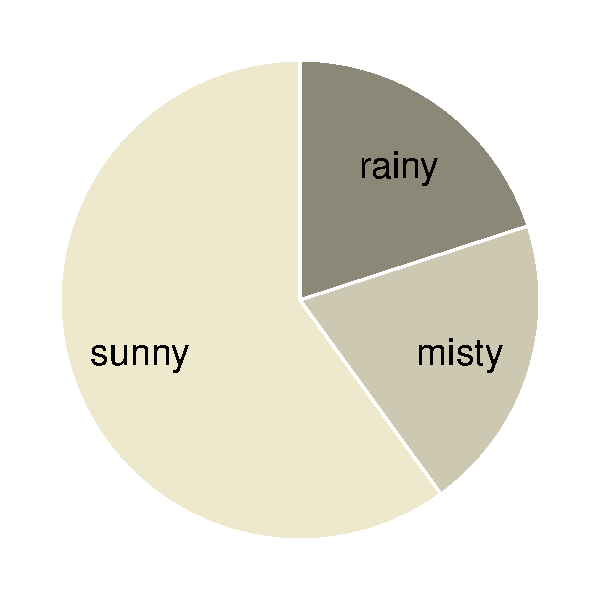
\includegraphics[width=0.9\textwidth]{00-pics/pie-chart-beliefs-Jones.pdf}
  \end{minipage}
  \hfill
  \begin{minipage}{0.45\linewidth}
    \centering
    \textbf{Smith}
    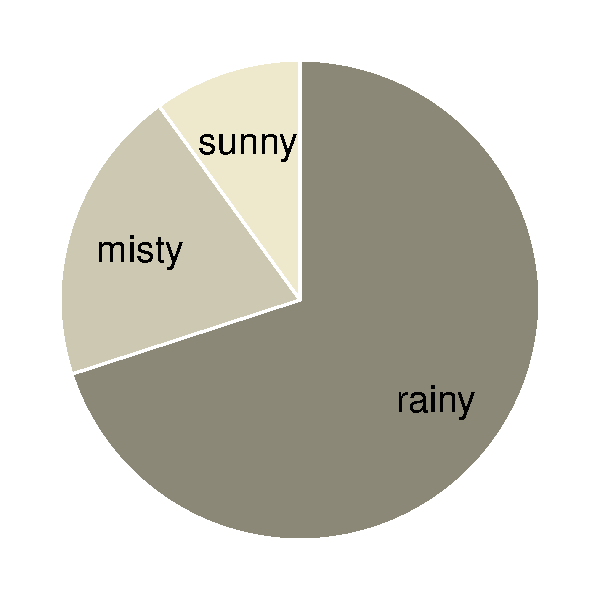
\includegraphics[width=0.9\textwidth]{00-pics/pie-chart-beliefs-Smith.pdf}
  \end{minipage}
  \caption{Two beliefs about the weather, represented as wheels of fortune.}
  \label{fig:belief-wheels}
\end{figure}

\subsection{Non-normalized probabilities}

Since what matters most are odds, not absolute numbers, we can also specify probability distributions in terms of non-normalized probabilities.
Concretely, the following is a complete and sufficient alternative way of specifying Jones' beliefs as in Table~\ref{tab:beliefs-weather}:
\begin{align*}
  P(\text{sunny})   & \propto 120
  & P(\text{misty}) & \propto 40
  & P(\text{rainy}) & \propto 40 &
\end{align*}
Here, the operator $\propto$ (read: ``proportional to'') is used.
More generally, if $f \colon \Omega \rightarrow \mathbb{R}^{\ge 0}$ is a function that maps each elementary outcome of $\Omega$ onto a non-negative real number, then writing $P(\omega) \propto f(\omega)$ fully and unambiguously defines a probability distribution in terms of the non-normalized probabilities assigned to each $\omega$ by $f$, namely:
\begin{align*}
  P(\omega) = \frac{f(\omega)}{\sum_{\omega'}f(\omega')}
\end{align*}


% example: P(x) \propto x^2 (for 1 \le x \le 5)


\subsection{Urns and frequencies}
\label{sec:urns-frequencies}

Another way of  thinking about probabilities for discrete sets $\Omega$, is in terms of urns.
Think of an urn as a container which contains a number of $N > 1$ balls. Balls can be of
different color. For example, let us suppose that our urn has $k > 0$ black balls and $N-k$
white balls. (There is at least one black and one white ball.) For a single random draw from
our urn we have: $\Omega_{\text{urn}} = \set{\text{white}, \text{black}}$.
Figure~\ref{fig:urn-3-7} shows such an urn with $k=7$ and $N=10$.


\begin{marginfigure}
  \centering
  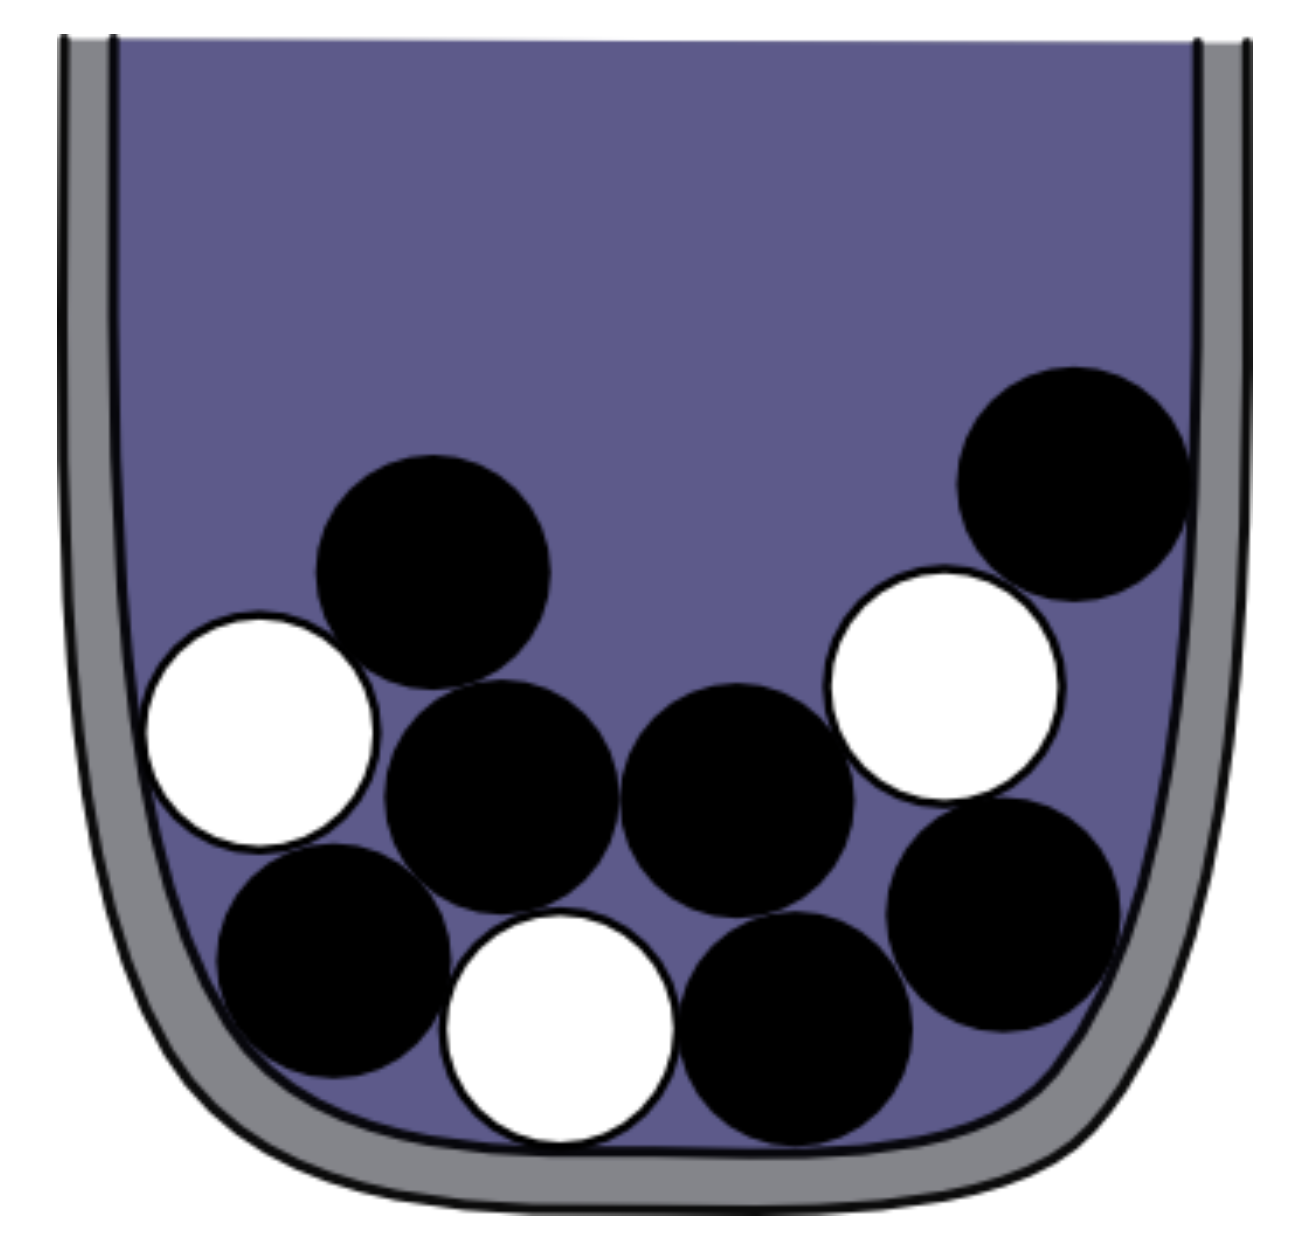
\includegraphics[width=0.7\textwidth]{00-pics/05-01-urn-3-7.png}
  \caption{Urn with $k=7$ black balls out of $N=10$ balls in total.}
  \label{fig:urn-3-7}
\end{marginfigure}

Imagine a long sequence of single draws from the urn in Figure~\ref{fig:urn-3-7}, putting whichever ball we drew back in after every draw.
We keep a record of how many times we drew a black ball, and divide this number by the number of times we drew a ball.
Figure~\ref{fig:limiting-frequencies} shows the results from a computer simulation of this process.
In general, the limiting proportion with which we draw a black ball is $\frac{k}{N}$.
Another way of saying this is that the \emph{objective} probability is $P(\text{black}) = \frac{k}{N}$.
Consequently, a rational agent's subjective beliefs should conform to the objective probability $P(\text{black}) = \frac{k}{N}$, unlike in other cases like the weather.

\begin{figure*}
  \centering
  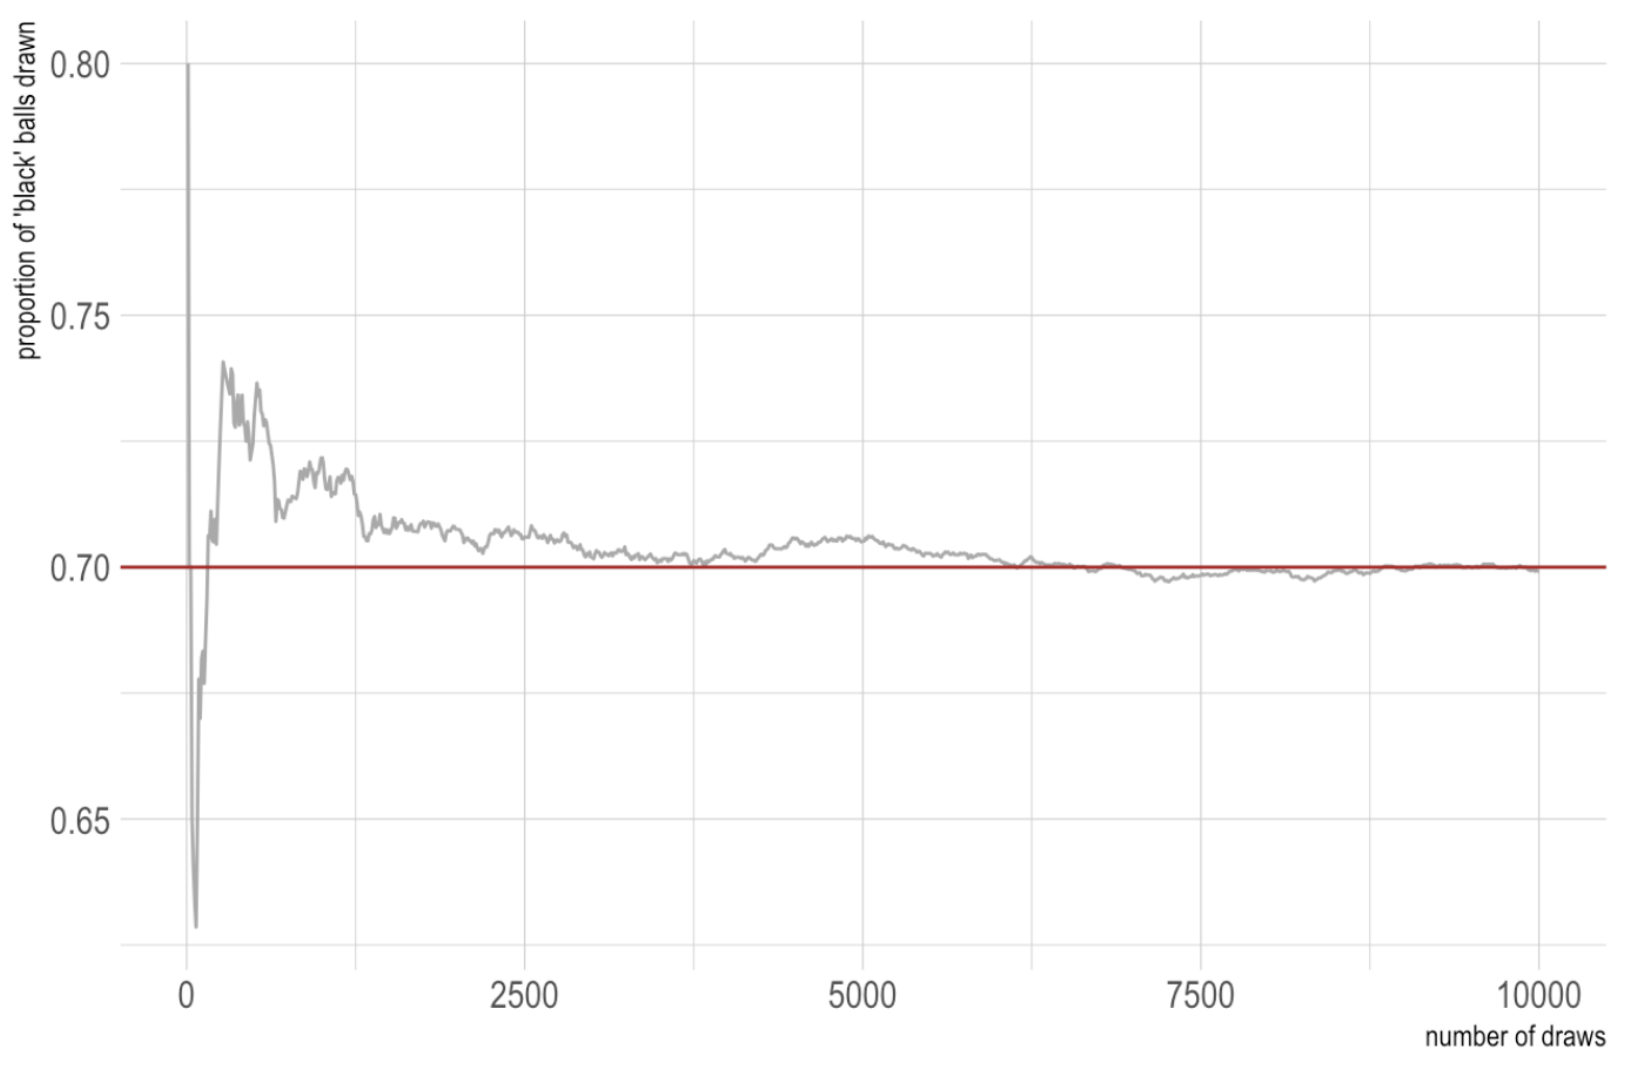
\includegraphics[width=0.8\textwidth]{00-pics/05-02-limiting-frequencies.png}
  \caption{Temporal development of the proportion of drawing a black ball from the urn.}
  \label{fig:limiting-frequencies}
\end{figure*}

\bigskip
\noindent \colorbox{mygray}{\centering
  \begin{minipage}{1.0\textwidth}

    \begin{exercise}
      Using the rules of probability theory, prove that the following claims hold.
      \begin{enumerate}[{C}1.]
        \item $P(\emptyset) = 0$
        \item $P(\overline{A}) = 1 - P(A)$
        \item $P(A \cup B) = P(A) + P(B) - P(A \cap B)$ for any $A, B \subseteq \Omega$
      \end{enumerate}
    \end{exercise}

    \begin{exercise}
      Write down the probability distributions over $\Omega_{\text{weather}} = \set{\text{sunny}, \text{misty}, \text{rainy}}$ that are defined in terms of the following pieces of information
      \begin{enumerate}[(i)]
        \item Miller believes that ``rainy'' is impossible, and that ``sunny'' is three times as likely as ``misty.''
        \item Ford has beliefs given by the following non-normalized probabilities:
        \begin{align*}
          P(\text{sunny})   & \propto 3
          & P(\text{misty}) & \propto 9
          & P(\text{rainy}) & \propto 27 &
        \end{align*}
        \item Johnson believes that ``sunny'' is as likely as not and that the odds in favor of ``rainy'' over ``misty'' are 3 to 2.
      \end{enumerate}

    \end{exercise}

  \end{minipage}
}

\newpage

\section{Structured events \& marginal distributions}

\subsection{Probability table for a flip-\&-draw scenario}

Suppose we have two urns. Both have $N=10$ balls. Urn 1 has $k_1=2$ black and $N-k_1 = 8$ white
balls. Urn 2 has $k_2=4$ black and $N-k_2=6$ white balls. We sometimes draw from urn 1,
sometimes from urn 2. To decide, we flip a fair coin. If it comes up heads, we draw from urn 1;
if it comes up tails, we draw from urn 2.
A schematic representation of this \emph{flip-\&-draw scenario} is shown in Figure~\ref{fig:flip-draw}.

\begin{figure}
  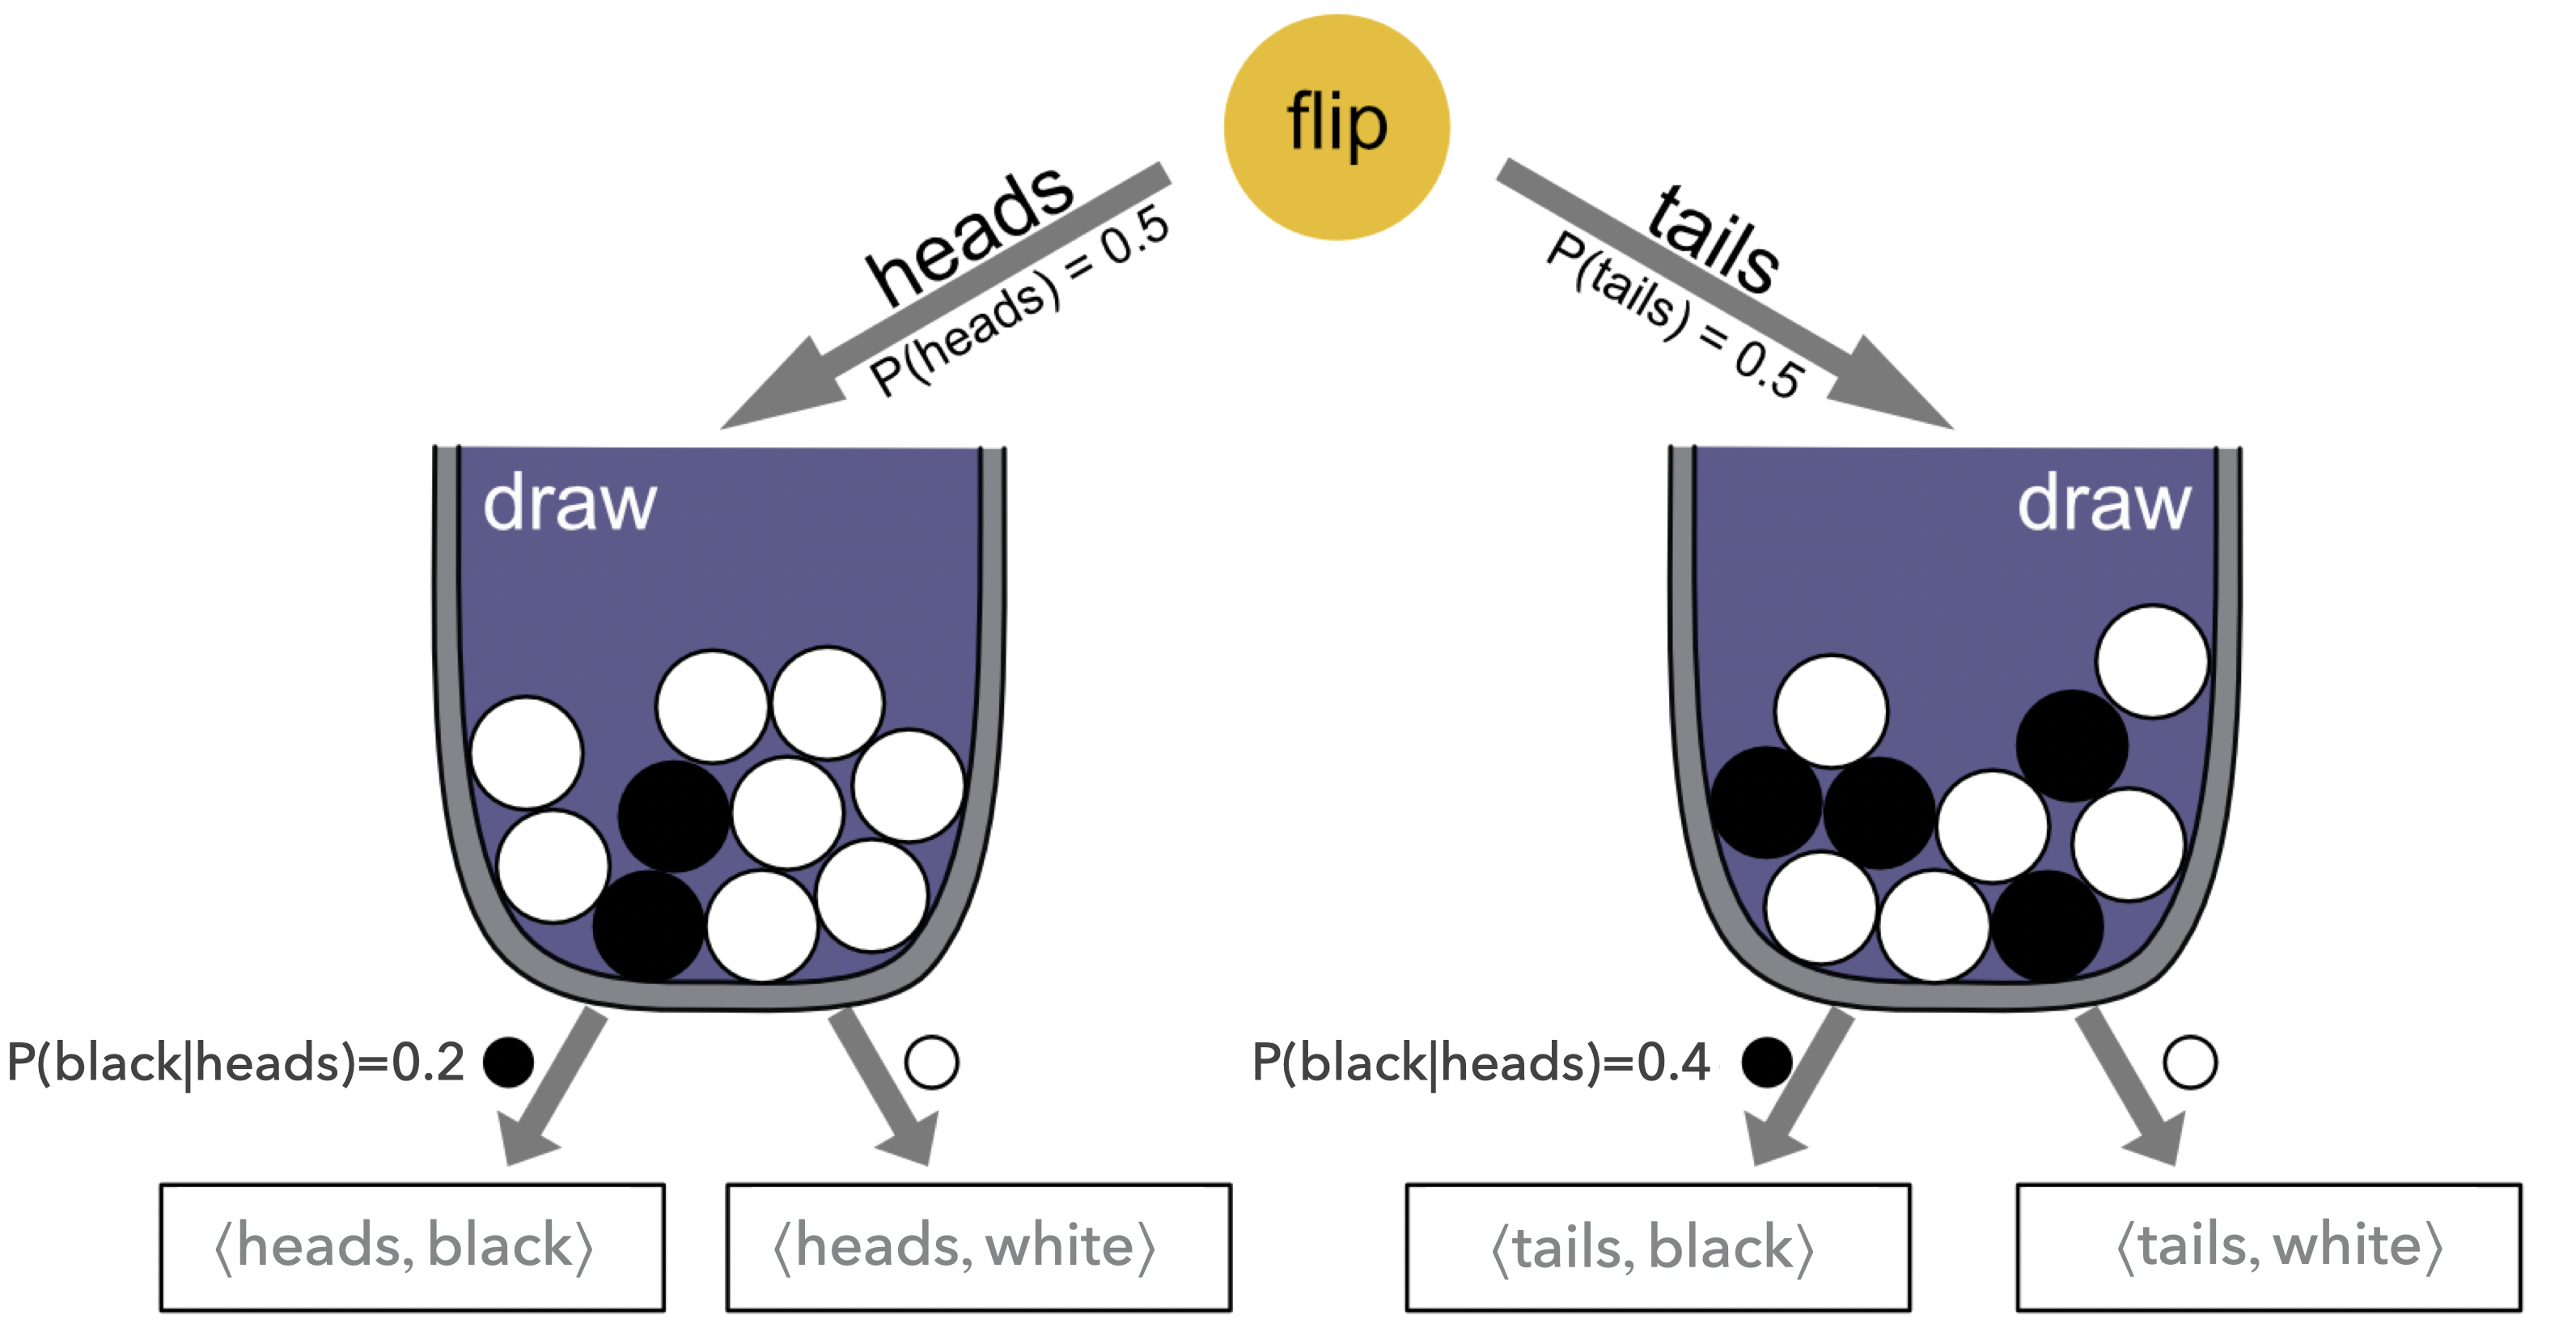
\includegraphics[width=1.0\textwidth]{00-pics/05-03-flip-draw.png}
  \caption{The flip-\&-draw scenario, illustrating structured event spaces and conditional probabilities.}
  \label{fig:flip-draw}
\end{figure}

An elementary outcome of this two-step process of flip-\&-draw is a pair
$\tuple{\text{outcome-flip}, \text{outcome-draw}}$.
The set of all possible such outcomes is
\begin{align*}
\Omega_{\text{flip-\&-draw}} & = \set{\tuple{\text{heads}, \text{black}}, \tuple{\text{heads},
    \text{white}}, \tuple{\text{tails}, \text{black}}, \tuple{\text{tails},
    \text{white}}}
\end{align*}
The probability of event $\tuple{\text{heads}, \text{black}}$ is given by
multiplying the probability of seeing ``heads'' on the first flip, which happens with
probability $0.5$, and then drawing a black ball, which happens with probability $0.2$, so that
$P(\tuple{\text{heads}, \text{black}}) = 0.5 \cdot 0.2 = 0.1$. The probability distribution
over $\Omega_{\text{flip-draw}}$ is consequently as in
Table~\ref{tab:flip-and-draw:probabilities}.\sidenote{If in doubt, start flipping \&
  drawing and count your outcomes.}
%
\begin{table}
  \centering
  \begin{tabular}{lcc}
    & black & white \\ \midrule
    heads & $0.5 \mult 0.2 = 0.1$  & $0.5 \mult 0.8 = 0.4$ \\
    tails & $0.5 \mult 0.4 = 0.2$  & $0.5 \mult 0.6 = 0.3$
  \end{tabular}
  \caption{Probabilities of elementary outcomes (pairs of $\tuple{\text{outcome-flip},
      \text{outcome-draw}}$) in the flip-\&-draw example.}
  \label{tab:flip-and-draw:probabilities}
\end{table}

\subsection{Structured events and joint-probability distributions}

Table~\ref{tab:flip-and-draw:probabilities} is an example of a \markdef{joint
  probability distribution} over a structured event space, which here has two dimensions. Since
our space of outcomes is the Cartesian product of two simpler outcome spaces, namely
$\Omega_{flip-\&-draw} = \Omega_{flip} \times \Omega_{draw}$,\sidenote{With
  $\Omega_{\text{flip}} = \set{\text{heads}, \text{tails}}$ and
  $\Omega_{\text{draw}} = \set{\text{black}, \text{white}}$.} we can use notation
$P(\text{heads}, \text{black})$ as shorthand for $P(\tuple{\text{heads}, \text{black}})$. More
generally, if $\Omega = \Omega_1 \times \dots \Omega_n$, we can think of $P \in \Delta(\Omega)$
as a joint probability distribution over $n$ subspaces.

\subsection{Marginalization}

If $P$ is a joint probability distribution over event space $\Omega = \Omega_1 \times \dots \Omega_n$, the \emph{marginal distribution} over subspace  $\Omega_i$, $1 \le i \le n$, is the probability distribution that assigns to all $A_i \subseteq \Omega_i$ the probability (where notation $P(\dots, \omega, \dots )$ is shorthand for $P(\dots, \{\omega \}, \dots)$):\sidenote{This notation, using $\sum$, assumes that subspaces are countable. In other cases, a parallel definition with integrals can be used.}

\begin{align*}
P(A_i) & = \sum_{\omega_1 \in \Omega_{1}} \sum_{\omega_2 \in \Omega_{2}} \dots  \sum_{\omega_{i-1} \in \Omega_{i-1}} \sum_{\omega_{i+1} \in \Omega_{i+1}} \dots \sum_{\omega_n \in \Omega_n} P(\omega_1, \dots, \omega_{i-1}, A_{i}, \omega_{i+1}, \dots \omega_n)
\end{align*}

For example, the marginal distribution over coin flips derivable from the joint probability
distribution in Table~\ref{tab:flip-and-draw:probabilities} gives $P(\text{heads}) = P(\text{tails}) =
0.5$, since the sum of each row is exactly $0.5$. The marginal distribution over flips
derivable from Table~\ref{tab:flip-and-draw:probabilities} has $P(\text{black}) = 0.3$ and
$P(\text{white}) = 0.7$.\sidenote{The term ``marginal distribution'' derives from such
  probability tables, where traditionally the sum of each row/column was written in the
  margins.}

\section{Conditional probability}

Fix probability distribution $P \in \Delta(\Omega)$ and events $A,B \subseteq \Omega$. The
conditional probability of $A$ given $B$, written as $P(A \mid B)$, gives the probability of
$A$ on the assumption that $B$ is true.\sidenote{We also verbalize this as ``the conditional
  probability of $A$ conditioned on $B$.''} It is defined like so:
\begin{align*}
  P(A \mid B) = \frac{P(A \cap B)}{P(B)}
\end{align*}
Conditional probabilities are only defined when $P(B) > 0$.\sidenote{
  Updating with events which have probability zero entails far more severe adjustments of the underlying belief system than just ruling out information hitherto considered possible.
  Formal systems that capture such \emph{belief revision} are studied in formal epistemology.
}


\begin{example}
  If a dice is unbiased, each of its six faces has equal probability to come up after a toss. The
  probability of event $B = \set{\epsdice{1}, \epsdice{3}, \epsdice{5}}$ that the tossed number
  is odd has probability $P(B) = \frac{1}{2}$. The probability of event $A = \set{\epsdice{3}, \epsdice{4},
    \epsdice{5}, \epsdice{6}}$ that the tossed number is bigger than two is $P(A) =
  \frac{2}{3}$. The probability that the tossed number is bigger than two \emph{and} odd is
  $P(A \cap B) = P(\set{\epsdice{3}, \epsdice{5}}) = \frac{1}{3}$. The conditional probability
  of tossing a number that is bigger than two, when we know that the toss is even, is $P(A \mid
  B) = \frac{\nicefrac{1}{3}}{\nicefrac{1}{2}} = \frac{2}{3}$.
\end{example}

Algorithmically, conditional probability first rules out all events in which $B$ is not true
and then simply renormalizes the probabilities assigned to the remaining events in such a way
that the relative probabilities of surviving events remains unchanged. Given this, another way
of interpreting conditional probability is that $P(A \mid B)$ is what a rational agent
\emph{should} believe about $A$ after observing that $B$ is in fact true and nothing more. The
agent rules out, possibly hypothetically, that $B$ is false, but otherwise does not change
opinion about the relative probabilities of anything that is compatible with $B$.

\subsection{Bayes rule}

Looking back at the joint-probability distribution in
Table~\ref{tab:flip-and-draw:probabilities}, the conditional probability
$P(\text{black} \mid \text{heads})$ of drawing a black ball, given that the initial coin flip
showed heads, can be calculated as follows:
\begin{align*}
  P(\text{black} \mid \text{heads}) = \frac{P(\text{black} , \text{heads})}{P(\text{heads})} =
  \frac{0.1}{0.5} = 0.2
\end{align*}
This calculation, however, is quite spurious. We knew that already from the way the
flip-\&-draw scenario was set up. After flipping heads, we draw from urn 1, which has $k=2$ out
of $N=10$ black balls, so clearly: if the flip is heads, then the probability of a black ball
is $0.2$. Indeed, in a step-wise random generation process like the flip-\&-draw scenario, some
conditional probabilities are very clear, and sometimes given by definition. These are,
usually, the conditional probabilities that define how the process unfolds forward in time, so
to speak.

\markdef{Bayes rule} is a way of expressing, in a manner of speaking, conditional probabilities in terms of the
``reversed'' conditional probabilities:
\begin{align*}
  P(B \mid A) = \frac{P(A \mid B) \mult P(B)}{P(A)}
\end{align*}
Bayes rule follows directly from the definition of conditional probabilities,
according to which $P(A \cap B) = P(A \mid B) \mult P(B)$, so that:
\begin{align*}
  P(B \mid A) = \frac{P(A \cap B)}{P(A)} = \frac{P(A \mid B) \cdot P(B)}{P(A)}
\end{align*}

Bayes rule allows for reasoning backwards from observed causes to likely underlying effects.
When we have a feed-forward model of how unobservable effects probabilistically constrain
observable outcomes, Bayes rule allows us to draw inferences about \emph{latent/unobservable
  variables} based on the observation of their downstream effects.

Consider yet again the flip-\&-draw scenario. But now assume that Jones flipped the coin and
drew a ball. We see that it is black. What is the probability that it was drawn from urn 1,
equivalently, that the coin landed heads? It is not $P(\text{heads}) = 0.5$, the so-called
\emph{prior probability} of the coin landing heads. It is a conditional probability, also
called the \emph{posterior probability},\sidenote{The terms \emph{prior} and \emph{posterior}
  make sense when we think about an agent's belief state before (prior to) and after (posterior
  to) an observation.} namely $P(\text{heads} \mid \text{black})$, but one
that is not as easy and straightforward to write down as the reverse
$P(\text{black} \mid \text{heads})$ of which we said above that it is an almost trivial part of
the set up of the flip-\&-draw scenario. It is here that Bayes rule has its purpose:
\begin{align*}
  P(\text{heads} \mid \text{black}) = \frac{P(\text{black} \mid \text{heads}) \mult P(\text{heads})}{P(\text{black})} =
  \frac{0.2 \mult 0.5}{0.3} = \frac{1}{3}
\end{align*}
This result is quite intuitive. Drawing a black ball from urn 2 (i.e., after seeing tails) is twice
as likely as drawing a black ball from urn 1 (i.e., after seeing heads). Consequently, after
seeing a black ball drawn, with equal probabilities of heads and tails, the probability that
the coin landed tails is also twice as large as that it landed heads.

\subsection{Stochastic (in-)dependence}

Event $A$ is \emph{stochastically independent} of $B$ if, intuitively speaking, learning $B$ does not change one's beliefs about $A$, i.e., $P(A \mid B) = P(A)$.

\begin{claim}
  If $A$ is stochastically independent of $B$, then $B$ is stochastically independent of $A$.
\end{claim}
\begin{proof}
  \begin{align*}
    P(B \mid A)
    & =
      \frac{P(A \mid B) \ P(B)}{P(A)} && \text{[Bayes rule]}
    \\
    & =
      \frac{P(A) \ P(B)}{P(A)} && \text{[by ass. of independence]}
    \\
    & =
      P(B) && \text{[cancellation]}
  \end{align*}
\end{proof}

For example, imagine a flip-and-draw scenario like in Figure~\ref{fig:flip-draw} where the initial coin flip has a bias of $0.8$ towards heads, but each of the two urns has the same number of black balls, namely $3$ black and $7$ white balls.
Intuitively and formally, the probability of drawing a black ball is then \emph{independent} of the outcome of the coin flip; learning that the coin landed heads, does not change our beliefs about how likely the subsequent draw will result in a black ball.
The probability table for this example is in Table~\ref{tab:joint-prob-independence}.

% ```{r flipdrawprobabilities-independent, echo = F}
% knitr::kable(
%   tibble(
%     " " = c("black", "white", "$\\Sigma$ columns"),
%     "heads" = c("$0.8 \\mult 0.3 = 0.24$", "$0.8 \\mult 0.7 = 0.56$", 0.8),
%     tails = c("$0.2 \\mult 0.3 = 0.06$", "$0.2 \\mult 0.7 = 0.14$", 0.2),
%     "$\\Sigma$ rows" = c(0.3, 0.7, 1)
%   ),
%   booktabs = T,
%   caption = 'Joint probability table for a flip-and-draw scenario where the coin has a bias of $0.8$ towards heads and where each of the two urns holds $3$ black and $7$ white balls.',
%   escape = F
% )
% ```

\begin{table}
  \centering
  \begin{tabular}{lccr}
                   &heads                    & tails                   & $\sum$ rows \\ \midrule
    black          & $0.8 \times 0.3 = 0.24$ & $0.2 \times 0.3 = 0.06$ & 0.3\\
    white          & $0.8 \times 0.7 = 0.56$ & $0.2 \times 0.7 = 0.14$ & 0.7 \\ \midrule
    $\sum$ columns & $0.8$                   & $0.2$
  \end{tabular}

  \caption{Joint probability table for a flip-and-draw scenario where the coin has a bias of $0.8$ towards heads and where each of the two urns holds $3$ black and $7$ white balls.}
  \label{tab:joint-prob-independence}
\end{table}

Independence shows in Table~\ref{tab:joint-prob-independence} in the fact that the probability in each cell is the product of the two marginal probabilities.
This is a direct consequence of stochastic independence:

\begin{claim}[Probability of conjunction of stochastically independent events]
  For any pair of events $A$ and $B$ with non-zero probability:
  \begin{align*}
    P(A \cap B) = P(A) \ P(B) \, \ \ \ \ \text{[if } A \text{ and } B \text{ are stoch. independent]}
  \end{align*}
\end{claim}

\begin{proof}
  By assumption of independence, it holds that $P(A \mid B) = P(A)$. But then:
  \begin{align*}
    P(A \cap B)
    & =
    P(A \mid B) \ P(B) && \text{[def. of conditional probability]}
    \\
    & =
    P(A) \ P(B) && \text{[by ass. of independence]}
  \end{align*}
\end{proof}

%%%%%%%%%%%%%%%%%%%%%%%%%
% exercises
%%%%%%%%%%%%%%%%%%%%%%%%%

\bigskip
\noindent \colorbox{mygray}{\centering
  \begin{minipage}{1.0\textwidth}

    \begin{exercise}
      Consider a flip-\&-draw scenario like the process in Figure~\ref{fig:flip-draw}, but with a biased coin that lands heads with probability 0.7.
      Assume further that the ``heads-urn'' (the urn to draw from after a ``heads'' outcome) has 25 balls in total out of which 10 are black, and that the ``tails-urn'' has 30 balls in total out of which 20 are black.
      \begin{enumerate}[(i)]
        \item Calculate the joint probability of all elementary outcomes (pairs of flips and draws).
        \item Compute the marginal probabilities of ``heads'' and ``tails.''
        \item Compute the conditional probability of ``heads'' given ``black.''
      \end{enumerate}
    \end{exercise}

    \begin{exercise}
      Consider the following (fictitious) joint-probability table of hair and eye color.

      \begin{tabular}{lcccc}
                   & black hair & brown hair & blonde hair & red hair \\ \midrule
        brown eyes & 0.4        & 0.22       & 0.05        & 0.03 \\
        blue eyes  & 0.05       & 0.12       & 0.08        & 0.004 \\
        green eyes & 0.001      & 0.01       & 0.005       & 0.03
      \end{tabular}

    \begin{enumerate}[(i)]
      \item Calculate the following marginal probabilities. (NB: This exercise uses informal notation like ``non-green eyes'' instead of cumbersome set-theoretic notation.)

      \begin{enumerate}[a.]
        \item $P(\text{black hair})$
        \item $P(\text{black hair or red hair})$
        \item $P(\text{non-green eyes})$
      \end{enumerate}

      \item Calculate the following conditional probabilities:

      \begin{enumerate}[a.]
        \item $P(\text{blue eyes} \mid \text{black hair})$
        \item $P(\text{brown hair} \mid \text{non-brown eyes})$
        \item $P(\text{non-green eyes} \mid \text{brown eyes})$
        \item $P(\text{black hair} \mid \text{blue eyes})$
      \end{enumerate}

      \item Which of the following events are stochastically independent?

      \begin{enumerate}[a.]
        \item black hair and green eyes
        \item black hair and brown hair
      \end{enumerate}

    \end{enumerate}
    \end{exercise}

    % \begin{exercise}
    %   Alex and Bo are Jones' children. Each child is allowed to take two sweets each day and they always do take exactly two sweets each. However, there is also a rule that says that the two sweets have to be different. Today Jones observes that three candy bars are missing and one lollipop. That means that one of the children must have taken the same sweet twice. Ha!

    %   Jones decides to test them. The first child to enter the living room will have to show the content of their right pocket. It turns out that this is Alex who shows Jones a chocolate bar. Should Jones conclude from this that Alex is more or less likely to be the culprit than Bo?

    %   Assume that it is, according to Jones, \emph{a priori} equally likely that either child would enter the living room first (whether they are the culprit or not). Assume also that the kids always have one sweet in one pocket, the other in the other pocket, but it is equally likely which sweet goes into which pocket. Model the situation in analogy to the flip-\&-draw scenario (children are coin flips, pockets are urns) and use Bayes rule to compute the probability that Alex is guilty given that Jones observed a chocolate bar in one of Alex's pockets.
    % \end{exercise}
  \end{minipage}
}

\newpage

\section{Random variables}

We have so far defined a probability distribution as a function that assigns a probability to
each subset of the space $\Omega$ of elementary outcomes.
A special case occurs when we are interested in a space of numeric outcomes, such as the probability of observing 3 heads when throwing a coin 10 times, or of measuring a reaction time of 300\,ms in a lexical decision task.
Probability distributions over numeric outcomes are conceptually no different from other probability distributions: in each case we set up a space of elementary outcomes as sets of possible worlds which agree on a certain criterion of relevance, which could be something non-numeric (like hair color) or numeric (like the integer or real valued reaction time in an experimental trial).
Yet, ``probability distributions over numbers'' are special because we often like to use mathematical operations in connection with the elementary outcomes or events.
For instance, we might be interested in the probability of numerical observations obtained by throwing a fair dice twice in a row and adding the number shown in each.
To express these kinds of operations and transformations, we use a special notation for ``probability distributions over numbers'' called \emph{random variables}.
\subsection{Definition, notation \& terminology}

A \markdef{random variable} is a function $X \mycolon \Omega \rightarrow \mathds{R}$ that
assigns to each elementary outcome a numerical value.
Traditionally, random variables are represented by capital letters, like $X$. Variables for the
numeric values they take on are written as small letters, like $x$.
We write $P(X = x)$ as a shorthand for the probability
$P(\set{\omega \in \Omega \mid X(\omega) = x})$ that an event occurs that is mapped onto $x$ by
random variable $X$. Similarly, we can also write $P(X \le x)$ for the probability
of observing an event that $X$ maps to a number not bigger than $x$.

If the range of $X$ is countable (not necessarily finite), we say that $X$ is \markdef{discrete}. For ease of exposition, we may say that if the range of $X$ is an interval of real numbers, $X$ is called \markdef{continuous}.\sidenote{
  This introductory primer only looks at the discrete case. The continuous case requires special mathematical treatment, but the underlying ideas behind central definitions and behavior are, for the most part, conceptually analogous.}

The \emph{support} of a random variable $X$ is:
\begin{align*}
  \text{support}(X) = \set{x \in \text{range}(X) \mid P(X = x) \neq 0}.
\end{align*}

When the context is clear enough, we might also just write $P(x)$ as a shorthand for $P(X = x)$.

\begin{example}
  \label{example:single-coin-RV}

  For a single flip of a coin we have $\Omega_{\text{coin flip}} = \set{\text{heads}, \text{tails}}$.
  A usual way of mapping outcomes of coin flips to numbers is to say that ``heads'' is 1 and ``tails'' is 0.
  The probability of an outcome depends on the bias $\theta$ which the coin has towards landing heads up.
  Therefore we define $X_{\text{flip}}^{\theta} \mycolon \text{heads} \mapsto 1; \text{tails} \mapsto 0$ and obtain that:
  \begin{align*}
    P(X_{\text{flip}}^{\theta} = 1) = \theta \ \ \ \ P(X_{\text{flip}}^{\theta} = 0) = 1-\theta
  \end{align*}
  Figure~\ref{fig:single-flip} shows examples of the probability distributions of single flips of a fair ($\theta = 0.5$) and a biased coin which lands heads three times more often than tails ($\theta=0.75$).
  The support of $X_{\text{flip}}^{\theta}$ is $\set{0,1}$ whenever $0 < \theta < 1$.

  \begin{figure}
    \centering
    \pgfplotstableread[row sep=\\,col sep=&]{
      xval                              & fair & biased \\
      0                                 & 0.5  & 0.25 \\
      1                                 & 0.5  & 0.75 \\
    }\singleCoinFlips

    \begin{tikzpicture}
      \begin{axis}[
        ybar,
        bar width=.5cm,
        width=4cm,
        height=4cm,
        % legend style={at={(0.5,1)},
        % anchor=north,legend columns=-1},
        % symbolic x coords={0,1},
        xtick=data,
        nodes near coords,
        % nodes near coords align={vertical},
        xmin=-0.5,xmax=1.5,
        ymin=-0,ymax=1,
        title={$P(X_{\text{flip}}^{0.5} = x)$},
        xlabel={$x$}
        ]
        \addplot[fill=mygray2] table[x=xval,y=fair]{\singleCoinFlips};
      \end{axis}
    \end{tikzpicture}
    \ \ \ \ \ \ \ \
    \begin{tikzpicture}
      \begin{axis}[
        ybar,
        bar width=.5cm,
        width=4cm,
        height=4cm,
        % legend style={at={(0.5,1)},
        % anchor=north,legend columns=-1},
        % symbolic x coords={0,1},
        xtick=data,
        nodes near coords,
        % nodes near coords align={vertical},
        xmin=-0.5,xmax=1.5,
        ymin=-0,ymax=1,
        title={$P(X_{\text{flip}}^{0.75} = x)$},
        xlabel={$x$}
        ]
        \addplot[fill=mygray2] table[x=xval,y=biased]{\singleCoinFlips};
      \end{axis}
    \end{tikzpicture}

    \caption{Probability distribution for random variables $X_{\text{flip}}^{0.5}$ (fair coin) and $X_{\text{flip}}^{0.75}$ (biased coin).}
    \label{fig:single-flip}
  \end{figure}


\end{example}

\begin{example}
  Less trivially, imagine flipping a coin two times. Elementary outcomes should be individuated by the outcome of the first flip and the outcome of the second flip, so that we get:
  \begin{align*}
    \Omega_{\text{2flips}} = \set{\tuple{\text{heads}, \text{heads}}, \tuple{\text{heads}, \text{tails}},
    \tuple{\text{tails}, \text{heads}}, \tuple{\text{tails}, \text{tails}}}
  \end{align*}
  Consider the random variable $X_{\text{2flips}}^{\theta}$ that counts the total number of heads.
  Crucially, we assign the same numerical value to different elementary outcomes, because $X_{\text{2flips}}^{\theta}(\tuple{\text{heads}, \text{tails}}) = 1 = X_{\text{two       flips}}(\tuple{\text{tails}, \text{heads}})$.
  Figure~\ref{fig:two-flips} shows examples for a fair ($\theta = 0.5$) and a biased coin which ($\theta=0.75$).
  The support of $X_{\text{2flips}}^{\theta}$ is $\set{0,1,2}$ whenever $0 < \theta < 1$.

  \begin{figure}
  \centering
  \pgfplotstableread[row sep=\\,col sep=&]{
    xval                              & fair & biased \\
    0                                 & 0.25  & 0.0625 \\
    1                                 & 0.5   & 0.375 \\
    2                                 & 0.25  & 0.5625 \\
  }\twoFlips

  \begin{tikzpicture}
    \begin{axis}[
      ybar,
      bar width=.5cm,
      width=6cm,
      height=4cm,
      % legend style={at={(0.5,1)},
      % anchor=north,legend columns=-1},
      % symbolic x coords={0,1},
      xtick=data,
      nodes near coords,
      % nodes near coords align={vertical},
      xmin=-0.5,xmax=2.5,
      ymin=-0,ymax=1,
      title={$P(X_{\text{2flips}}^{0.5} = x)$},
      xlabel={$x$}
      ]
      \addplot[fill=mygray2] table[x=xval,y=fair]{\twoFlips};
    \end{axis}
  \end{tikzpicture}
  \hfill
  \begin{tikzpicture}
    \begin{axis}[
      ybar,
      bar width=.5cm,
      width=6cm,
      height=4cm,
      % legend style={at={(0.5,1)},
      % anchor=north,legend columns=-1},
      % symbolic x coords={0,1},
      xtick=data,
      nodes near coords,
      % nodes near coords align={vertical},
      xmin=-0.5,xmax=2.5,
      ymin=-0,ymax=1,
      title={$P(X_{\text{2flips}}^{0.75} = x)$},
      xlabel={$x$}
      ]
      \addplot[fill=mygray2] table[x=xval,y=biased]{\twoFlips};
    \end{axis}
  \end{tikzpicture}

  \caption{Probability distribution for random variables $X_{\text{2flips}}^{0.5}$ (fair coin flipped twice, count number of heads) and $X_{\text{2flips}}^{0.75}$ (same for biased coin landing ``heads'' three times more often than ``tails'').}
  \label{fig:two-flips}
\end{figure}

\end{example}

% \subsection{Cumulative distribution \& density of a continuous random variable}

% For a continuous random variable $X$, the probability $P(X = x)$ will usually be zero: it is
% virtually impossible that we will see precisely the value $x$ realized in a random event that
% can realize uncountably many numerical values of $X$. However, $P(X \le x)$ does take workable
% values and so we define the \markdef{cumulative distribution function} $F_X$
% associated with $X$ as a primitive (i.e., as given by definition):
% \begin{align*}
%   F_X(x) = P(X \le x)
% \end{align*}
% Instead of a probability \emph{mass} function, we derive a \markdef{probability density
%   function} from the cumulative function as:
% \begin{align*}
%   f_X(x) = F'(x)
% \end{align*}
% A probability density function can take values greater than one, unlike a probability mass
% function.

% \begin{example}
%   The \markdef{Gaussian or Normal distribution} characterizes many natural distributions of
%   measurements which are symmetrically spread around a central tendency. It is defined as:
%   \begin{align*}
%     \mathcal{N}(X = x ; \mu, \sigma) = \frac{1}{\sqrt{2 \sigma^2 \pi}} \exp \left ( -
%       \frac{(x-\mu)^2}{2 \sigma^2} \right)
%   \end{align*}
%   where parameter $\mu$ is the \emph{mean}, the central tendency, and parameter $\sigma$ is the
%   \emph{standard deviation}. Figure~\ref{fig:NormalDistribution} gives examples of the
%   probability density function of two normal
%   distributions. Figure~\ref{fig:NormalDistributionCumulative} gives the corresponding
%   cumulative distribution functions.

% \begin{figure}
%   \centering
%   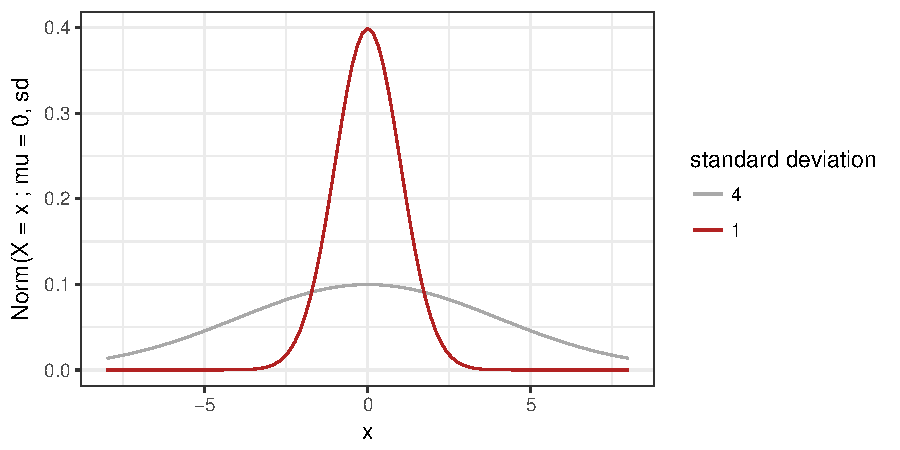
\includegraphics[width=\textwidth]{00-pics/05_01_normal-distribution.pdf}
%   \caption{Examples of the Normal distribution. In both cases $\mu = 0$, once with $\sigma = 1$
%     and once with $\sigma = 4$.}
%   \label{fig:NormalDistribution}
% \end{figure}

% \begin{figure}
%   \centering
%   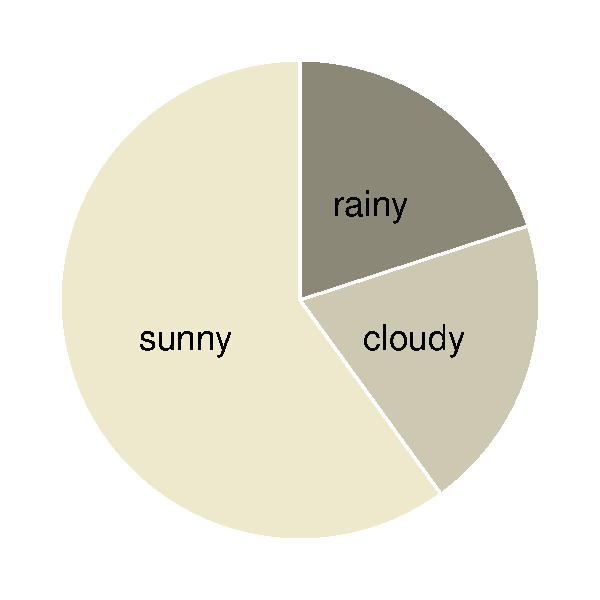
\includegraphics[width=\textwidth]{00-pics/05_01_normal-distribution-cumulative.pdf}
%   \caption{Examples of the cumulative normal distribution corresponding to the previous probability
%     density functions.}
%   \label{fig:NormalDistributionCumulative}
% \end{figure}

% \end{example}

\subsection{Expected value}

The \markdef{expected value of random variable} $X$ (a.k.a.~the \emph{mean} of $X$) is a measure of central tendency.
It tells us, like the name suggests, which average value of $X$ we can expect when repeatedly sampling from $X$.
If $X$ is discrete, the expected value is:
\begin{align*}
  \mathds{E}_X = \sum_{x \in \text{support}(X)} x \mult P(X = x)
\end{align*}

\begin{example}
  The expected values of $X_{\text{flip}}^{\theta}$ is:
  \begin{align*}
    \mathds{E}_{X_{\text{flip}}^{\theta}} = \sum_{x \in \text{support}(X_{\text{flip}}^{\theta})} x \mult P(X = x) = (1- \theta) \mult 0 + \theta \mult 1 = \theta
  \end{align*}
  So, concretely, for a fair coin we have $\mathds{E}_{X_{\text{flip}}^{0.5}} = 0.5$.
  This show that the expected value is not (necessarily) the same as the most likely value.
\end{example}

The \markdef{expected value of function} $f \mycolon \mathbb{R} \rightarrow \mathbb{R}$ under $X$ is:\sidenote{This will be useful for the definition of information-theoretic notions, such as \emph{entropy}.}
\begin{align*}
  \mathds{E}_X = \sum_{x \in \text{support}(X)} f(x) \mult P(X = x)
\end{align*}


\subsection{Composite random variables}

The notation in terms of random variables is particularly useful for composite random variables, when we write expressions like $Z = 2X + Y$.
For instance, $X_{\text{flip}^{\theta}}$ might be the outcome of a single flip of a coin with bias $\theta$ (as in Example~\ref{example:single-coin-RV}).
The composite variable $Z = X_{\text{flip}^{\theta}} + X_{\text{flip}^{\theta}}$ is built by, intuitively speaking, repeatedly generating random number from $X_{\text{flip}^{\theta}}$, and another one (independently) from $X_{\text{flip}^{\theta}}$ again and then adding the two numbers.
Indeed, the resulting composite random variable is what we already saw above:
\begin{align*}
  X_{\text{2flips}^{\theta}} = X_{\text{flip}^{\theta}} + X_{\text{flip}^{\theta}}
\end{align*}

\begin{figure}
  \centering
  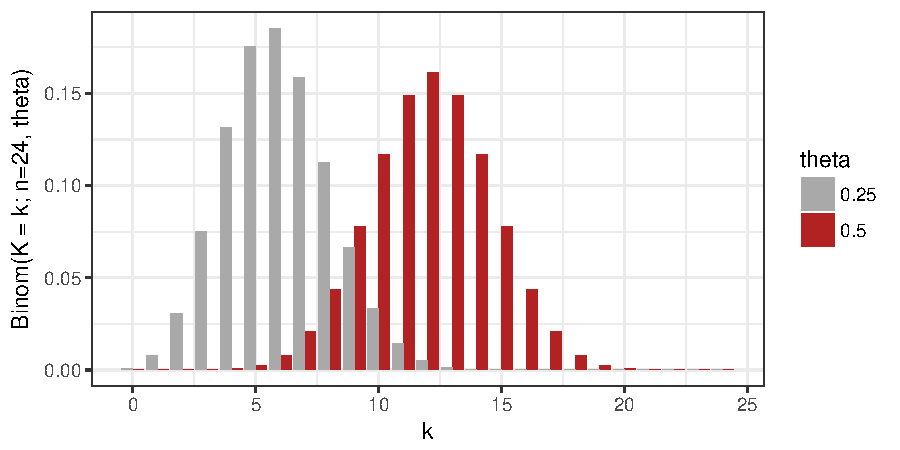
\includegraphics[width=\textwidth]{00-pics/05_00_binomial-distribution.pdf}
  \caption{Examples of the Binomial distribution. The $y$-axis give the probability of seeing
    $k$ heads when flipping a coin $n=24$ times with a bias of either $\theta = 0.25$ or
    $\theta = 0.5$.}
  \label{fig:BinomialDistribution}
\end{figure}

\begin{example}
  Let us generalize flipping coins and counting heads to more than 2 flips.
  The composite random variable $K^{n,\theta}$, with:
  \begin{align*}
    K^{n,\theta} = \underbrace{X_{\text{flip}^{\theta}} + \dots + X_{\text{flip}^{\theta}}}_{n \text{ times}}
  \end{align*}
  captures the total number of heads obtained from $n$ independent flips of a coin with bias $\theta$.
  The resulting probability distribution $P(K^{n,\theta}=k)$ is well-known and is called the \markdef{Binomial distribution}.
  We can express it with an elegant formula:\sidenote{
    Here $\binom{n}{k} = \frac{n!}{k!(n-k)!}$ is the binomial coefficient.
    It gives the number of possibilities of drawing an unordered set with $k$ elements from a set with a total of $n$ elements.
  }
  \begin{align*}
    P(K^{n,\theta}=k) = \text{Binom}(K = k ; n, \theta) = \binom{n}{k} \,  \theta^{k} \, (1-\theta)^{n-k}
  \end{align*}
  Figure~\ref{fig:BinomialDistribution} gives an example of the Binomial distribution for two values of the coin's bias, $\theta = 0.25$ or $\theta = 0.5$, when flipping the coin $n=24$ times.


\end{example}
Composite random variables need not just iterate the same random process.
\begin{example}
  Let $X$ be the probability distribution of rolling a fair dice with six sides.
  $Y$ is the probability distribution of flipping a biased coin that lands heads (represented as number 1) with probability 0.75.
  We are interested in the composite random variable $Z = X + Y$.
  The support of $Z$ is $\set{0, 1, \dots, 7}$.
  The probability mass function of $Z$ is show in Figure~\ref{fig:composite-RV}.
  \begin{figure}
    \centering
    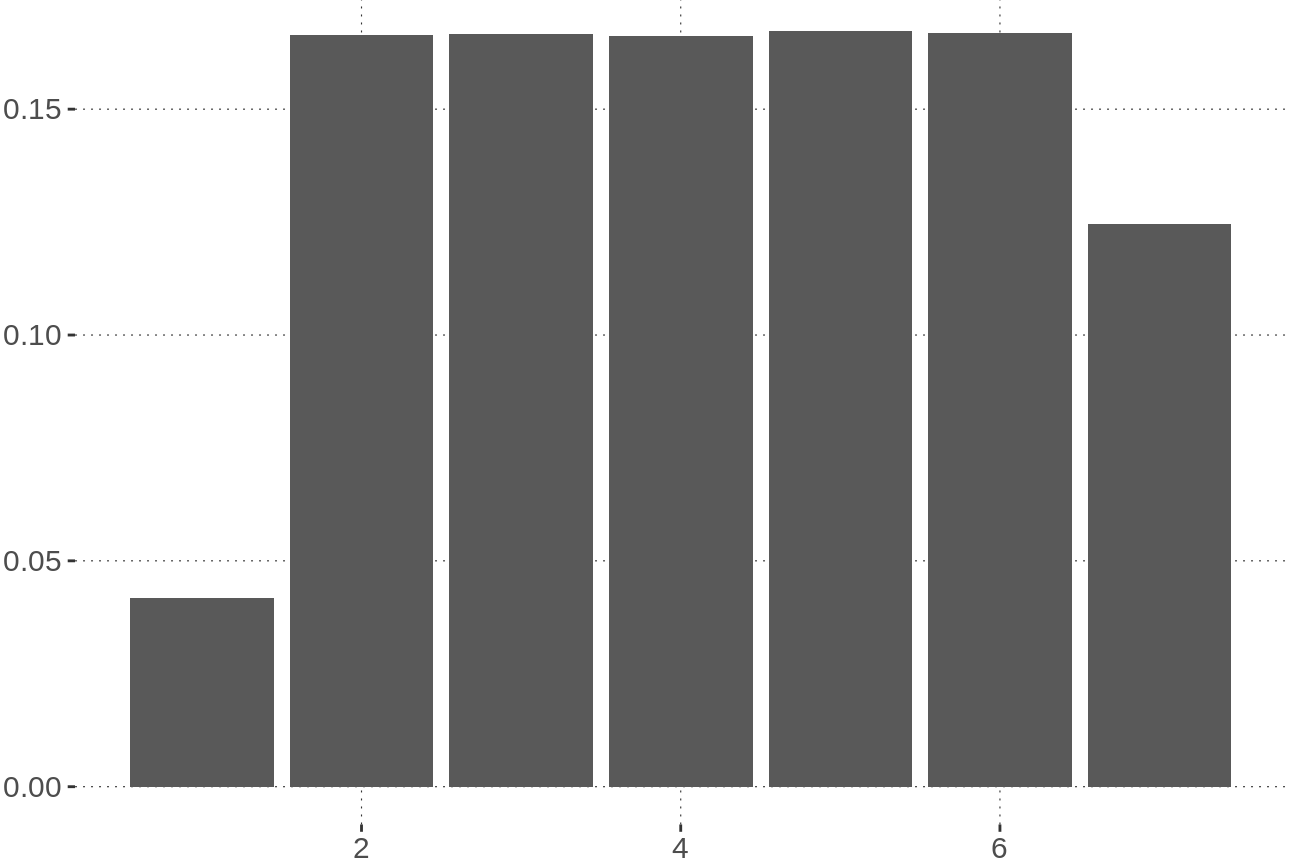
\includegraphics[width=0.9\textwidth]{00-pics/05-04-mass-composite-RV.png}
    \caption{Probability mass function of a random variable obtained by flipping a fair coin and adding the (numerical) outcome to the outcome of throwing a fair dice.}
    \label{fig:composite-RV}
  \end{figure}
\end{example}

Of course, more fancy mathematical operations, beyond summation, are conceivable, e.g.: $Z = \log(\abs{X}) - \sqrt{Y}$.
Notice, however, that there are some subtle differences with normal mathematical operations.
The variable $Y = 2 \mult X$ is not the same as $Z = X + X$ (see exercises below).

\bigskip
\noindent \colorbox{mygray}{\centering
  \begin{minipage}{1.0\textwidth}

    \begin{exercise}
      Let $X_{\text{dice}}$ be the random variable that maps each roll of a fair six-sided dice onto its numerical outcome.
      \begin{enumerate}
        \item What is the support of $X_{\text{dice}}$?
        \item Write down, for each $n$ in the support of $X_{\text{dice}}$, the probability $P(X_{\text{dice}}=n)$.
        \item What is the expected value of $X_{\text{dice}}$?
      \end{enumerate}
    \end{exercise}

    \begin{exercise}
      Let $Z = X_{\text{dice}} + X_{\text{dice}}$ be the composite random variable obtained by adding the number of two (independent) rolls of a fair six-sided dice.
      \begin{enumerate}
        \item What is the support of $Z$?
        \item Write down, for each $n$ in the support of $Z$, the probability $P(Z=n)$.
        \item What is/are the most likely outcome(s)? What is/are the least likely?
        \item What is the expected value of $Z$?
      \end{enumerate}
    \end{exercise}

    \begin{exercise}
      Let $Y = 2 \mult X_{\text{dice}}$ be the composite random variable obtained by throwing a fair six-sided dice once and multiplying the outcome by 2.
      \begin{enumerate}
        \item What is the support of $Y$?
        \item Write down, for each $n$ in the support of $Y$, the probability $P(Y=n)$.
        \item What is/are the most likely outcome(s)? What is/are the least likely?
        \item What is the expected value of $Y$?
      \end{enumerate}
    \end{exercise}

  \end{minipage}
}


% \printbibliography

\end{document}
